%%
%% This is file `thesis-ex.tex',
%% generated with the docstrip utility.
%%
%% The original source files were:
%%
%% uiucthesis2009.dtx  (with options: `example')
%% 
\def\fileversion{v2.25a} \def\filedate{2009/10/10}
%% Package and Class "uiucthesis2009" for use with LaTeX2e.
\documentclass[edeposit,10pt,fullpage]{uiucthesis2009}

\usepackage{amsmath, amsthm, amssymb}
\usepackage[numbers]{natbib}

\usepackage{color}
\usepackage{verbatim}

\usepackage{subfigure}
\usepackage{url}
\usepackage{times}
\usepackage{mathptmx}
\usepackage[ruled,vlined]{algorithm2e}
\usepackage[pdftex]{graphicx}
\usepackage{booktabs}

\usepackage{subfigure}
\usepackage{caption}
\usepackage{tikz}
\usetikzlibrary{arrows,positioning,fit,scopes}
\usetikzlibrary{shapes.multipart}

\colorlet{d}{black!25}
\colorlet{l}{black!0}
\newcommand{\btnode}[4]{ \nodepart{#1} #2\\ $[$#3,#4) }
\newcommand{\btplainnode}[2]{ \nodepart{#1} #2  \\  }
\tikzset{nd/.style={rectangle split, rectangle split parts=3, draw=black!75, thick,
            rectangle split horizontal, align=center, rectangle split empty part width=0.5cm,
            rectangle split part fill={#1}}}

\usepackage[pdfborder={0 0 0}]{hyperref}

\interfootnotelinepenalty=10000  % Split footnote are annoying

\newcommand{\ntaskip}{\vspace{-0.15in}}
\SetAlgoSkip{ntaskip}

\newenvironment{captiontext}{%
   \begin{center}%
     \begin{minipage}{0.99\linewidth}%
       \renewcommand{\baselinestretch}{0.9}%
         \sffamily\footnotesize}%
   {\renewcommand{\baselinestretch}{1.0}%
      \end{minipage}%
        \end{center}}

\newenvironment{smitemize}%
  {\begin{list}{$\bullet$}%
     {\setlength{\parsep}{0pt}%
      \setlength{\topsep}{0pt}%
      \setlength{\itemsep}{2pt}}}%
  {\end{list}}

\clubpenalty=10000  % Don't allow orphans
\widowpenalty=10000 % Don't allow widows

% \raggedbottom

\renewcommand{\textfraction}{0}
\renewcommand{\topfraction}{1}
\renewcommand{\bottomfraction}{1}
\setcounter{totalnumber}{10}
\setcounter{topnumber}{10}
\setcounter{bottomnumber}{10}
\setcounter{dbltopnumber}{10}
\renewcommand{\floatpagefraction}{1}
\renewcommand{\dblfloatpagefraction}{1}

%Remove this at the end.
\newcommand{\citetemp}[1]{(#1)}
\newcommand{\temp}[1]{?#1?}

\begin{document}

\title{System and Framework for Identification of Info Malware on the Android Operating System}
\author{Robert Marsan}
\department{Computer Science}
\schools{M.S, University of Illinois at Urbana-Champaign, 2013}
\msthesis
\advisor{Roy H. Campbell}
\degreeyear{2013}
\committee{Professor Roy H. Campbell}
\maketitle

\frontmatter

%% Create an abstract that can also be used for the ProQuest abstract.
%% Note that ProQuest truncates their abstracts at 350 words.
\begin{abstract}
The tremendous rise of mobile computing has led to an equally strong rise in mobile malware. We address this issue with several novel concepts, permission fingerprints and user-app agreements. We also present a groundbreaking and substantial new dataset of the state of Android Apps, and provide unique results gathered from it. Finally, we present AndroMEDA, an Android Security Extension which helps address many of the shortcomings to existing techniques of malware identification currently available.


This $seriously$ needs to be extended.

\end{abstract}

%% Create a dedication in italics with no heading, centered vertically
%% on the page.
\begin{dedication}
To my\\
Parents, Lisa and Mark
\end{dedication}

%% Create an Acknowledgements page, many departments require you to
%% include funding support in this.
\chapter*{Acknowledgments}

I would like to thank my advisor Roy H. Campbell for his mentorship and guidance, as well as Alejandro Gutierrez for putting up with me.

%% The thesis format requires the Table of Contents to come
%% before any other major sections, all of these sections after
%% the Table of Contents must be listed therein (i.e., use \chapter,
%% not \chapter*).  Common sections to have between the Table of
%% Contents and the main text are:
%%
%% List of Tables
%% List of Figures
%% List Symbols and/or Abbreviations
%% etc.

\tableofcontents
\listoftables
\listoffigures
\listofalgorithms

%this can add another section...?
%\addcontentsline{toc}{chapter}{List of Algorithms}

%% Create a List of Abbreviations. The left column
%% is 1 inch wide and left-justified
%\chapter{List of Abbreviations}
%
%\begin{symbollist*}
%\item[CA] Caffeine Addict.
%\item[CD] Coffee Drinker.
%\end{symbollist*}

%% Create a List of Symbols. The left column
%% is 0.7 inch wide and centered
%\chapter{List of Symbols}

%\begin{symbollist}[0.7in]
%\item[$\tau$] Time taken to drink one cup of coffee.
%\item[$\mu$g] Micrograms (of caffeine, generally).
%\end{symbollist}

\mainmatter
\chapter{Introduction}
\label{sec:intro}

%\textbf{Thesis Statement}: Malware, and especially Info Theft Malware, on Mobile Operating Systems, especially Android, is better understood when not just analyzing the capabilities of an application, but the expectations the user has as to how it utilizes those capabilities as well.\\
%\textbf{Thesis Statement}: Android Malware detection is complemented by not just analyzing the capabilities of an app, but the context and use as well.\\
%\textbf{Thesis Statement}: In order to detect Android Malware, the user must understand what is going on behind the scenes of the app. The capabilities of an app are important, but the context and use of these capabilities are as well.\\
\textbf{Thesis Statement}: Using a novel feedback loop, we provide users with a method for understanding the context and use of actions an app performs, thus allowing them to identify suspicious behavior that violates users' trust.\\


The rise of smartphones in the last decade years has been unprecedented. Since the launch of the Apple iPhone in 2007, there are now almost 1 Billion smartphone users in the world\citep{kpcbinternetreport2012}. These new devices marked an unprecedented shift in our relationship with computers, becoming the center point for many personal endeavors, and superseding almost all previous computing devices from cell phones, to cameras, to GPS devices, and to most uses of a desktop PC\citep{hua2012introduction}. Smartphones continue to become the focal point of almost all personal computing, and consequently the operating systems they run become more important and powerful.

\section{Contributions}
In this thesis, we highlight 4 key areas:
\begin{smitemize}
\item \textit{User-App Agreement}: First, we discuss the challenges of addressing modern mobile malware, and the shortcomings of the Android security model. We introduce the User-App Agreement (UAA), a way of conceptualizing the trust a user has in actions an applications may perform, as a key component in identifying malicious behavior.
\item \textit{Android Census}: Second, we use a novel dataset, Android Census, to examine the state of Android permissions. We find Android permissions correlate with expected use, but key examples are shown of less than legitimate use. Using a comprehensive set of malware, we cross examine how the permissions of malware compares with the Android Census. We conclude that malware that targets the user's personal information is the most difficult to detect using this static analysis.
\item \textit{IncognitoWare}: Third, we address the shortcomings of the current malware datasets available to academia, and introduce a new dataset of IncognitoWare. This dataset is more representative of current trends in malware, and proves to be a great challenge to detect.
\item \textit{AndroMEDA}: Finally, we introduce Android Malware Evaluation Detection and Analysis (AndroMEDA), a set of Android extensions, and a companion app, build off of the premise of the User-App Agreement. By giving the user more information on the context and use of sensitive system actions, they can evaluate whether they trust those actions, and ultimately whether the app is acting maliciously or not.
\end{smitemize}
\subsection{}





% After untrusted behavior is spotted, the actions can be reported, and knowledge can be spread to all users. All of this makes users more aware of app behavior, and helps mitigate Info Theft Malware on Android.

%Building off the concept of the User-App Agreement, we introduce AndroMEDA. Key parts of the User-App Agreement were previously unnoticable to the user until AndroMEDA. By giving the user more information on the context and use of permissions, they can evaluate whether they trust those actions, and ultimately whether the app is acting maliciously or not. After untrusted behavior is spotted, the actions can be reported, and knowledge can be spread to all users. All of this makes users more aware of app behavior, and helps mitigate Info Theft Malware on Android.


%This security model has dramatically changed the nature of mobile software, and in turn, mobile malware. By forcing malware to fit inside of this security sandbox, malware authors must choose to either break out of the box, or work inside of it. This constriction has blurred the definition of mobile malware, and ultimately has profound implications for the user of the mobile device. We will examine these implications, and propose new tools and methods to help understand the nuances of modern malware, as well as provide a framework of tools to detect them.


\chapter{Background \& Motivation}
\label{sec:background}

%To understand the nature of modern mobile malware, we first examine the context. The two main models, that of iOS and Android, are compared and contrasted here.

\section{The ``App'' and Sandboxing}

In the mobile world, ``Apps'' are isolated and sandboxed programs, generally designed with one singular purpose. They lack dependencies, and generally are not as privileges as system software for performing many tasks. The mechanisms for accessing functionality outside of their sandbox is enforced by a set of policies the system holds, specific to that app. On some platforms, like iOS, only one app may run at any given time, and background computation is virtually non-existent (with some exceptions)\footnote{Minor amounts of computation can be done to compute background audio, and other isolated background tasks.}, along with many other restrictions. On Android and other platforms, many more features are available to apps, but in all cases, the ``app'' lifecycle is well defined and controlled by the system much more than on a PC OS.

There are various reasons for the tight sandboxing of mobile apps. Power and resource consumption are certainly a factor - mobile OSs generally reserve the right to kill apps if they attempt to allocate too much memory. Controlling access to hardware also helps in this: allowing apps to keep the phone awake could easily drain battery. However, another reason for sandboxing, and arguably more important, is protecting Personally Identifiable Information.

\subsection{Personally Identifiable Information}

Personally Identifiable Information (PII), as defined by the National Institute of Standards and Technology, is ``any information about an individual maintained by an agency, including (1) any information that can be used to distinguish or trace an individual‘s identity... and (2) any other information that is linked or linkable to an individual'' \citep{mccallister2010guide}. Mobile devices, having blended cameras, cell phones, GPS devices, and PCs into one device, have an extremely diverse amount of PII, from phone numbers, to contacts, to location history, to bank account numbers and pictures. For many of these datasets, mobile OSs actually organize them into databases with the intention of allowing 3rd parties access to them. Contact lists, SMS, Photographs and location history are available to apps on virtually every mobile platform in some official way. This is a driving motivation for a greatly improved security model for mobile OSs: controlling 3rd party software's access to PII. 

% Expand more on this.

\subsection{Digital Distribution Platform}

The final major difference between mobile OSs and PC OSs is the distribution of code. No mobile OS allows 3rd party code to be ran outside of the sandbox, and all of them require the user's consent before installing an app. All apps must be signed, and in general, there is 1 main distribution channel for all apps on a mobile OS. This tightly controlled distribution both aids in security, as well as controls the ecosystem around that mobile OS.

\subsection{Apple's App Store}
The first major digital distribution platform for mobile apps was Apple's App Store\citep{AppleAppStore}. It's model has been repeated by almost all major mobile app distribution platforms. The basic premise is simple: developers sign up to the app store, pay a fee (usually yearly), and submit fully-finished apps. A reviewer runs the app in a monitored sandbox, watches for unusual behavior, checks for stability and usability, and approves it. Once the app has been approved, it's released onto the app store, at which time anyone can download it. The approval process, as well as the high monetary fee, act as a way to ensure only safe and high-quality apps are available for that platform. In this type of platform, typically no apps may be installed from other sources. On iOS, initially this was the main method of security: if the app passed the inspection, it was acknowledged as safe and virtually unmonitored unless someone noticed something unusual and reported it. However, in recent years, after certain incidents (see section \ref{sec:path}), apps still must request permission from the user to perform certain tasks.

\subsection{Android Permissions}
Android's distribution platform takes a different approach, and at it's core is also Android's security model: The Permission System (see section \ref{sec:permissions}). Android Apps declare when they are packaged what capabilities they will use, and the user reviews them at install time. If the user approves the app, it may use the requested capabilities whenever it wants: little restrictions are placed otherwise. With this barrier in mind, the Google Play Store (formerly known as the Android Market), or GPStore, opts for an alternate model to iOS, where the developer pays a smaller fee, and apps go through no formal approval process. After an app's submission, it's immediately released into the wild for users to download and run. The assumption Android uses is that the metadata the GPStore provides: App name, Developer Name, Description, Reviews and Ratings, are enough for the user to determine if the app should be trusted with the permission set it's given (see Figure \ref{fig:gpstoreapps}). In fact, Android even allows the device to accept apps from 3rd party sources, a practice known as ``sideloading'', although it's disabled by default. This has spawned a large number of 3rd party app sources, all of which rely on the Permission system for user protection.

%GPSTORE IMAGE AND CHART EXPLAINING THE LETTERS.

\begin{figure}[h]
\begin{center}
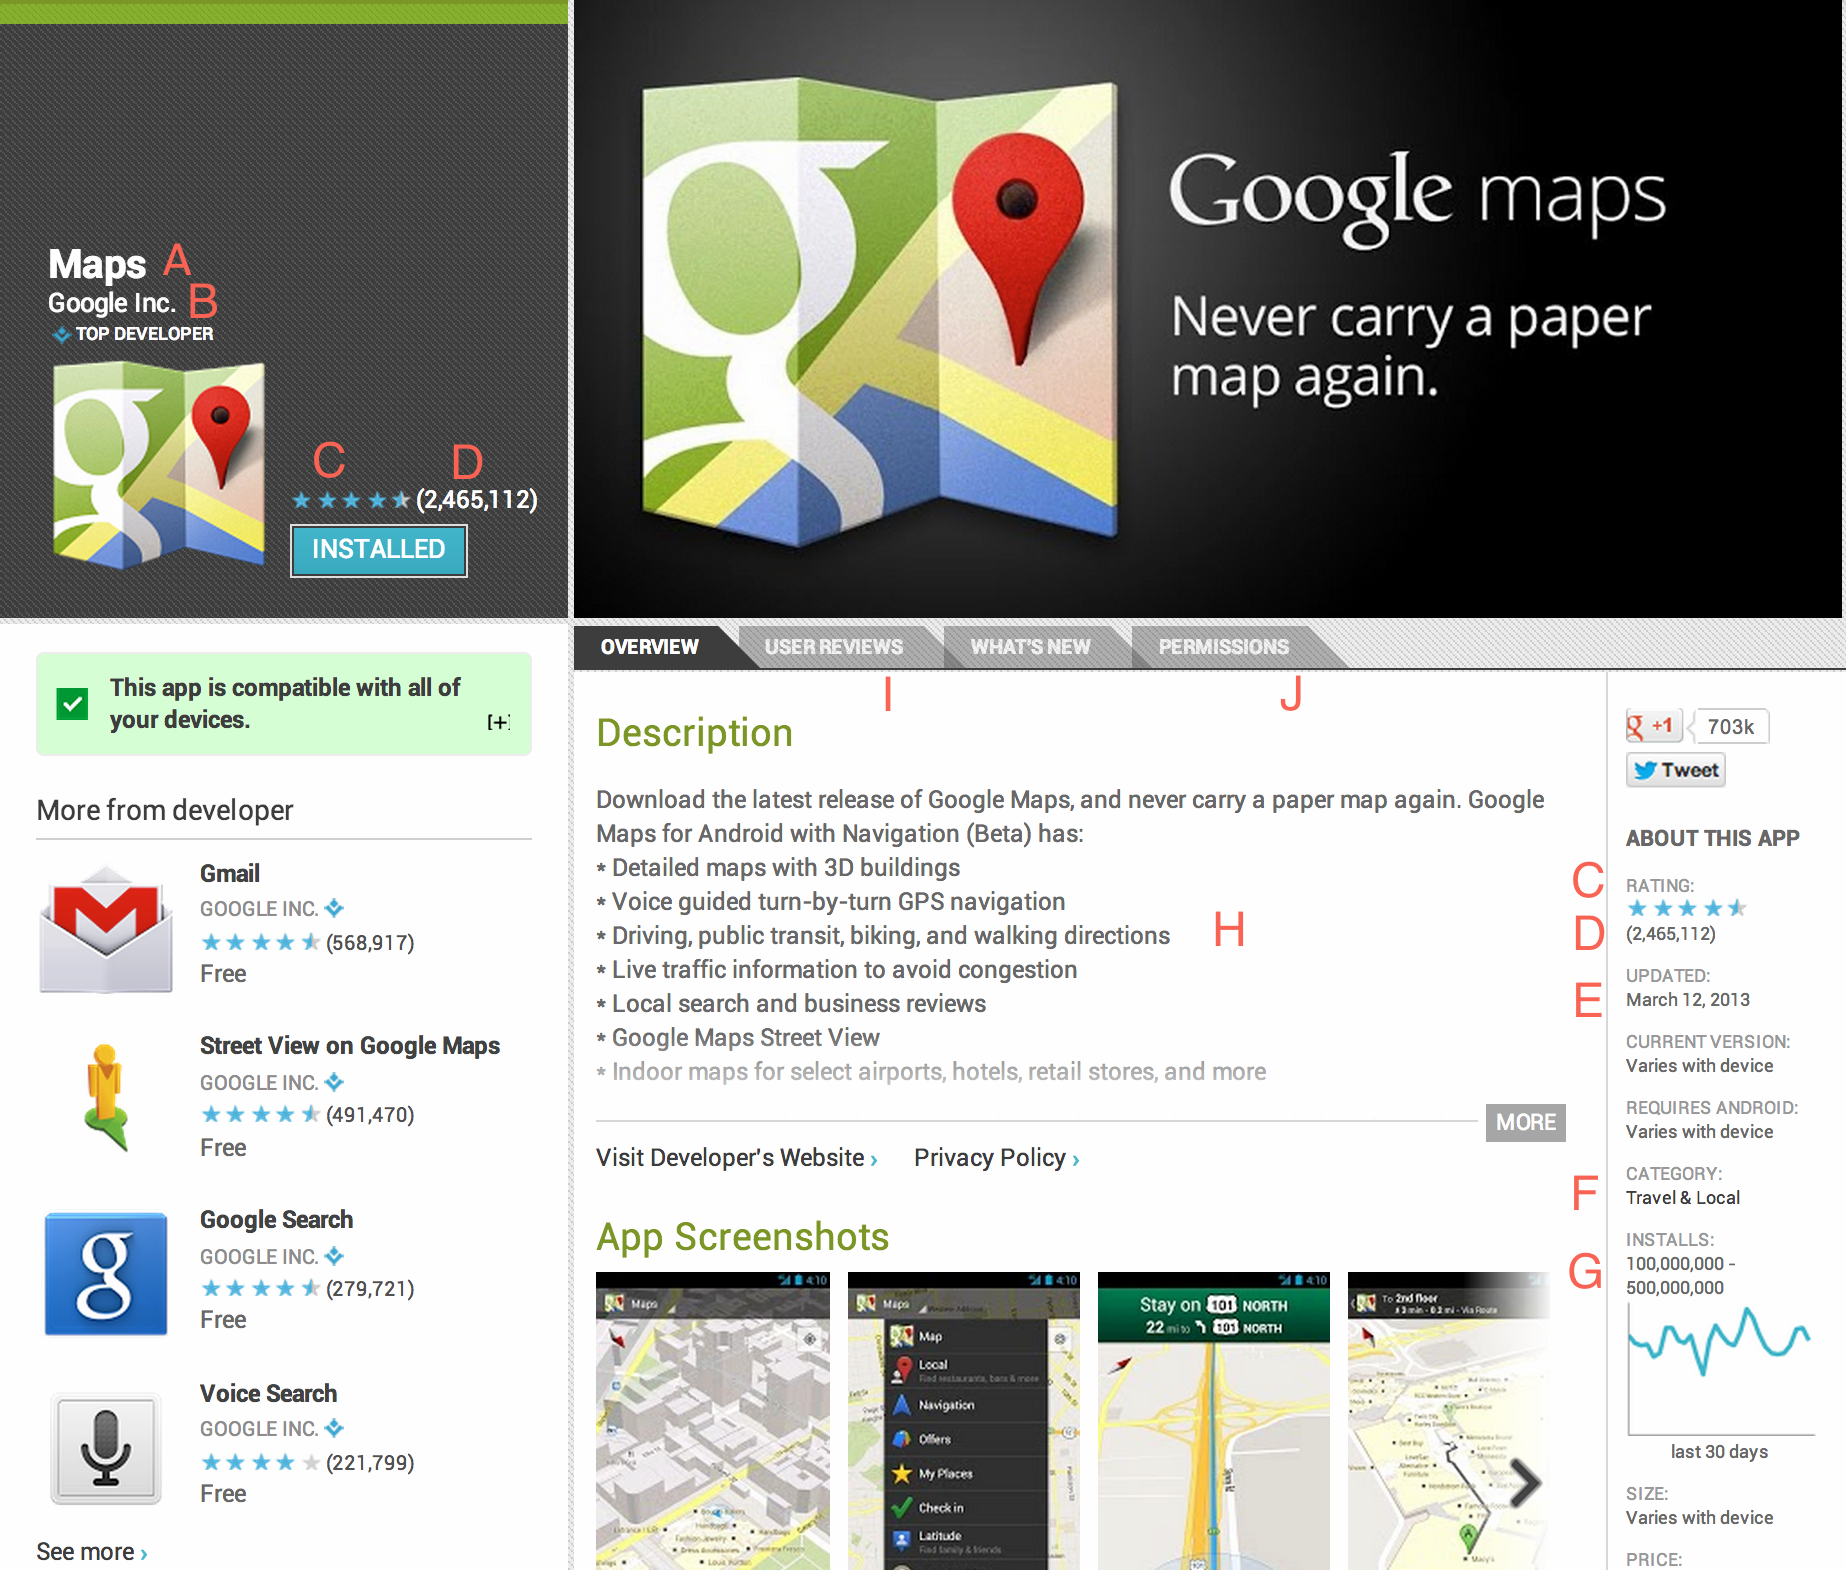
\includegraphics[width=0.9\columnwidth]{figs/GPStoreAppPage}
\caption{A sample page on the Google Play Store, see \ref{tab:gpstorekey}}
\label{fig:gpstoreapps}
\end{center}
\end{figure}

\begin{table*}[h]
\begin{small}
\begin{tabular}{l|l}

\textit{A} & App name  \\
\textit{B} & Developer Name  \\
\textit{C} & App Rating  \\
\textit{D} & Number of ratings  \\
\textit{E} & Date the app was last updated  \\
\textit{F} & Category in the Google Play Store it falls under  \\
\textit{G} & Number of installs (range, not exact number)  \\
\textit{H} & Description of the app  \\
\textit{I} & Reviews of the app  \\
\textit{J} & Permissions the app requests  \\

\end{tabular}
\end{small}
%\vspace{-0.2in}
\caption{Various properties of a Google Play Store app page}
\label{tab:gpstorekey}
%\vspace{-0.1in}
\end{table*}

%The core concept behind Android security - Permissions - are a static contract of capabilities. However, in this paper we propose an alternate means of conceptualizing security, which focuses on the interrelationship between the user's perception of the app, and the app's actual behavior. We call this the ``user-app agreement'', and will elaborate on it more later. 

\section{Malware}
Malware, as defined by the US Department of Homeland Security, is ``Short for malicious software. Programming (code, scripts, active content, and other software) designed to disrupt or deny operation, gather information that leads to loss of privacy or exploitation, gain unauthorized access to system resources, and other abusive behavior'' \citep{nash2005undirected}. Like PC OSs, malware is present on mobile OSs, although there are differences.


\subsection{Mobile Malware}
The tighter security model of Mobile OSs has a notable effect on mobile malware. With tight control in sandboxing, and app distribution, the usual viruses, trojans, and other exploits are more difficult to employ. The main vectors are either OS-level exploits, sneaking past the app review process, or through sideloading of apps. When looking at the two main mobile OSs, a stark contrast is shown. iOS has had  ``jailbreaking'' - privilege escalation exploits - dating back from it's first release \citep{damopoulos2011isam}, whereas the first Android exploit was not discussed until 2010 by security researchers Papathanasiou and Percoco \citep{papathanasiou2010not}, and was not seen in the wild until early 2011\citep{castillo2010android}. On the contrary, no side-loading is possible for iOS, and there have been very few - if any - instances of malware sneaking past Apple's App Store review process, although it has happened\footnote{In July 2012, SecureList noticed an iOS app that uploaded all of the user's contacts to a remote location without their consent\citep{SecureList2012}, but others argued this was not as devious as made out to be\citep{trendmicroios2012} }. With 95\% of all mobile malware\citep{nq2013}, Android's malware situation is very much a product of the sideloading and lack of review process found in GPStore\citep{nq2013}. %Of all the mobile malware found for iOS and Android, over \temp{some percent} used no system-exploits at all, \temp{some percent} on the main app distribution platform.

 On mobile devices, one of the dominant goals of malware is to gather information that leads to loss of privacy, found in over 28\% of mobile malware in 2012 alone\citep{nq2013}. This trend, of malware that possesses no system exploits, but gathers information that leads to loss of privacy, known as Info Theft Malware, is one that Android's Permission-based security model is ill-equipped to handle. Android's permission system relies on the user to determine at install-time if a list of capabilities should be entrusted with the given app. The user is not given a say in how or when the capabilities may be used, nor the ability to reject specific capabilities. At the same time, the mechanisms that keep mobile OSs safe are forcing malware writers to use more subtle techniques, often times without exploits. This all works against the user.

In this paper, we attempt to address this key issue through various means. We first introduce several novel concepts for analyzing apps and malware on Android. We then analyze the state of Android apps and Permissions with the most comprehensive android app database available, Android Census. Finally, we propose several novel improvements to the Android security architecture, called AndroMEDA, aimed at building off of our conceptual work.


\chapter{Conclusion and Future Work}
\label{sec:conclusion}
\section{Conclusion}
AndroMEDA helps users understand the context in which their Personally Identifiable Information is used, which allows them to make more informed decisions on whether an app is action maliciously or not. 

In this paper, we introduced 3 key items:
\subsection{User-App Agreement}
%We analyze the state of Android and Permissions, and conclude the need to address the User-App Agreement, which is a framework for consenting and trusting specific actions an app may take. It lies at the heart of classifying Info Theft Malware. Android Permissions address the capabilities of an app, but fail to address the context and use of those capabilities, which are cruicial to trusting an app's actions.

We analyzed the current Android security framework: The Permission System, and found it's main flaws were it's lack of addressing context and use, which we generalize into the User-App Agreement - a framework for consenting and trusting specific actions an app may take. Whereas Android Permissions exceeded at defining general capabilities of an app, and these capabilities go a long way in shaping the User-App Agreement, they fail at addressing the context in which the permissions are used, and what they are used for.

\subsection{\temp{AndroidMarketDB}}
To perform a full analysis of the current state of Android Permissions, we use a novel dataset, \temp{AndroidMarketDB}. By analyzing more than 80\% of apps in the Google Play Store, we are able to better understand the interrelationship of permissions and expected behavior. We produce key insights as to the popularity of apps vs their PII permissions, and when apps deviate from their expected behavior - potentially violating the User-App Agreement. We then analyze a comprehensive malware dataset using the same techniques, and find that many types of malware can be identified purely by it's permission fingerprint. We conclusively show the connection between Permissions and Expected Behavior are present, but not strong enough to differentiate between Info Theft Malware and many popular apps.

\subsection{AndroMEDA}
Building off the concept of the User-App Agreement, we introduce AndroMEDA. Key parts of the User-App Agreement were previously unnoticable to the user until AndroMEDA. By giving the user more information on the context and use of permissions, they can evaluate whether they trust those actions, and ultimately whether the app is acting maliciously or not. This, in turn, helps mitigate Info Theft Malware on Android.

\section{Future Work}
\label{sec:futurework}
AndroMEDA is, ultimately, not a silver bullet at detecting all Android malware. Projects like TaintDroid and TISSA provide functionality that would greatly enhance the abilities of AndroMEDA to visualize context and use of permissions to the user, and allow them to take action against it. 

AndroMEDA could also benefit greatly from the probablistic modeling of pBMDs and Crowdroid, in correlating user action with permission behavior. These would not replace the need to alert the user, but rather be able to better dictate when to put different classes of alerts to the user, as ultimately the decision of what is malware is up to them.

The weath of data in \temp{AndroidMarketDB} was also not fully explored. We are currently interested in seeing if specific keywords in user reviews correlate with malicious software, or other problematic apps. Many more areas of metadata, like the description, developer, etc, can be further explored, to see if it gives additional insight into the nature of malware on Android.

\appendix*

%\include{Appendix.tex}

\backmatter

\bibliographystyle{abbrvnat}
%\bibliographystyle{latex8}
\bibliography{ref}

\end{document}
\endinput
%% End of file `thesis-ex.tex'.
